\section{Results}

\subsection{Qualitative Results for the Filtering}
In our analysis of exiting behavior, the comparative visualizations between unfiltered Fig. ~\ref{fig:unfiltered} and filtered Fig. ~\ref{fig:filtered} datasets illuminate the impact of the filtering module. The unfiltered dataset, while comprehensive, includes noise and irrelevant data points that can obscure critical patterns of exiting behaviour. Conversely, Fig. ~\ref{fig:filtered}, representing the filtered dataset, showcases a more refined view, where additional information is eliminated, and the relevant behavioural patterns are emphasized. This clarity enhances our ability to precisely identify and analyse exiting manoeuvres, demonstrating the filtering module's efficacy in isolating meaningful data, thus improving the accuracy of our predictive models.

\begin{figure}[htbp]
    \centering
    \begin{minipage}[b]{0.45\columnwidth}
        \centering
        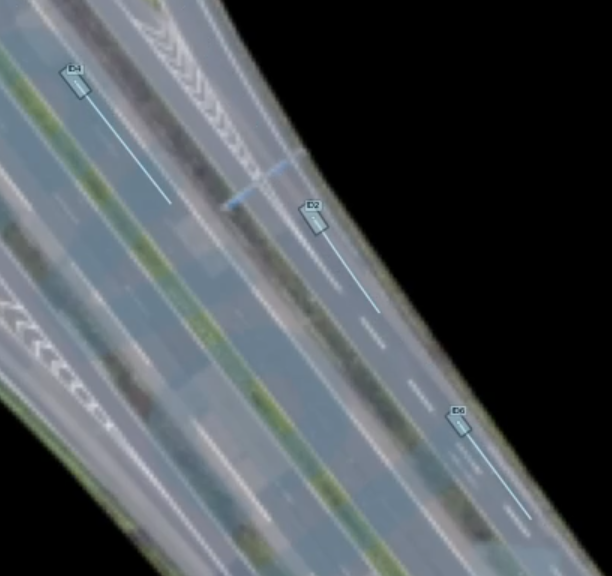
\includegraphics[width=\columnwidth]{images/figures/Filtering1.png}
        \caption{Unfiltered Exiting Scenario}
        \label{fig:unfiltered}
    \end{minipage}
    \hfill
    \begin{minipage}[b]{0.45\columnwidth}
        \centering
        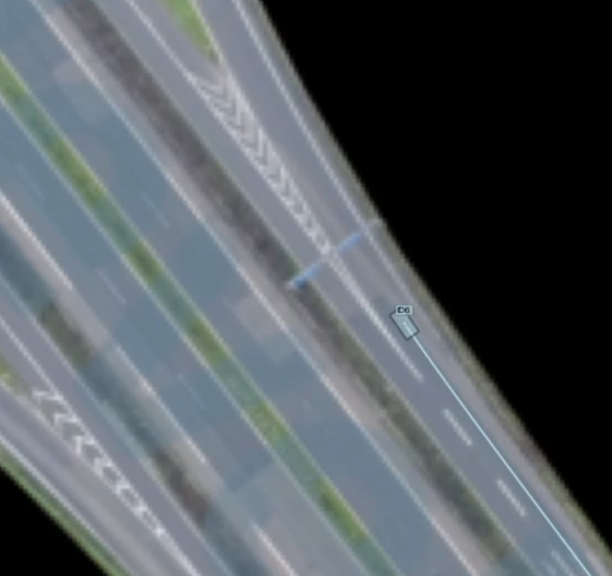
\includegraphics[width=\columnwidth]{images/figures/Filtering2.png}
        \caption{Filtered Exiting Scenerio}
        \label{fig:filtered}
    \end{minipage}
    \label{fig:cfiltered}
\end{figure}

Similar to the analysis of exiting behaviour, the comparison between unfiltered and filtered datasets for entering behaviour, depicted in Fig. ~\ref{fig:filtered2} and Fig. ~\ref{fig:unfiltered2}, respectively, offers insightful observations. The unfiltered dataset, depicted in Figure Fig. ~\ref{fig:filtered2}, presents a raw, comprehensive view of vehicle movements, including a mix of relevant and irrelevant behaviours for entering scenarios. ~\ref{fig:filtered2}, on the other hand, reveals the effectiveness of the filtering module in enhancing data clarity.

\begin{figure}[htbp]
    \centering
    \begin{minipage}[b]{0.45\columnwidth}
        \centering
        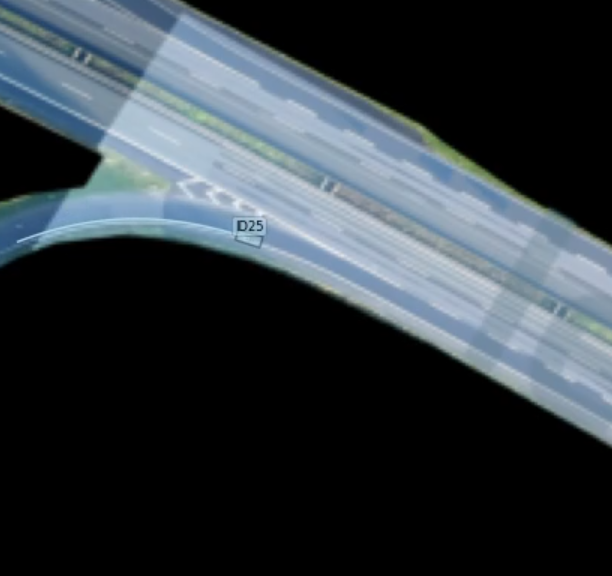
\includegraphics[width=\columnwidth]{images/figures/Filtering3.png}
        \caption{Unfiltered Entering Scenario}
        \label{fig:unfiltered2}
    \end{minipage}
    \hfill
    \begin{minipage}[b]{0.45\columnwidth}
        \centering
        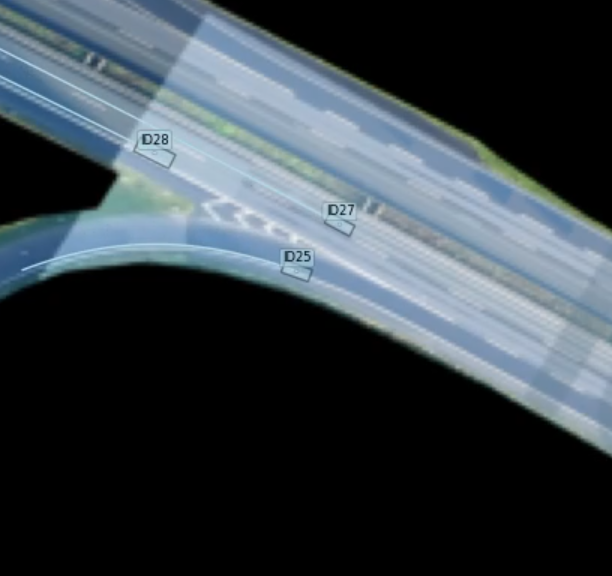
\includegraphics[width=\columnwidth]{images/figures/Filtering4.png}
        \caption{Filtered Entering Scenario}
        \label{fig:filtered2}
    \end{minipage}
    \label{fig:cfiltered2}
\end{figure}

\subsection{Linear Model}

The linear models that predict the acceleration derived from the distance formula
(\ref{eq:lin_model_acc_dis}) and the model derived from the velocity formula (\ref{eq:lin_model_acc_vel}) solved using linear regression have the following test results:


\begin{table}[h]
\centering
\caption{Comparison Results: Distance Model and Velocity Model}
\label{tab:model_comparison}
\begin{tabular}{l S[table-format=1.4e-2] S[table-format=1.4e-2] S[table-format=1.4e-2]}
\toprule
 & {MSE} & {MAE} & {$R^2$ Score} \\
\midrule
Distance Model & 3.5392e-03 & 1.1892e-02 & 9.8918e-01 \\
Velocity Model & 3.5370e-03 & 1.1877e-02 & 9.8918e-01 \\
\bottomrule
\end{tabular}
\end{table}

We can see that the predictions for the test set for both models are quite accurate having a very small MSE and MAE. 
We can also plot our results into graphs to have a better visual understanding of our results 
in figure \ref{fig:prediciton_acceleration_distance} and \ref{fig:prediciton_acceleration_velocity}.

\begin{figure}[h]
    \centering
    \begin{minipage}[b]{0.45\columnwidth}
        \centering
        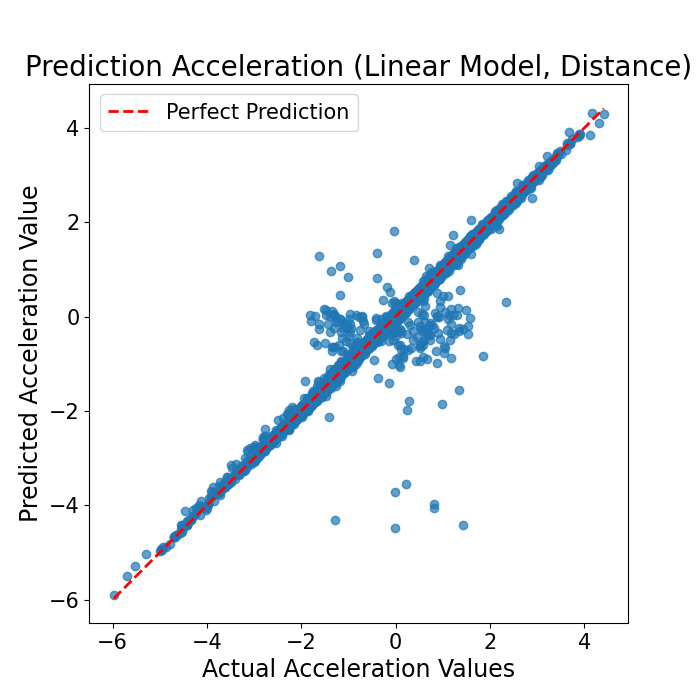
\includegraphics[width=\columnwidth]{images/figures/Prediction Acceleration (Linear Model, Distance).png}
        \caption{Prediction results Distance Model}
        \label{fig:prediciton_acceleration_distance}
    \end{minipage}
    \hfill
    \begin{minipage}[b]{0.45\columnwidth}
        \centering
        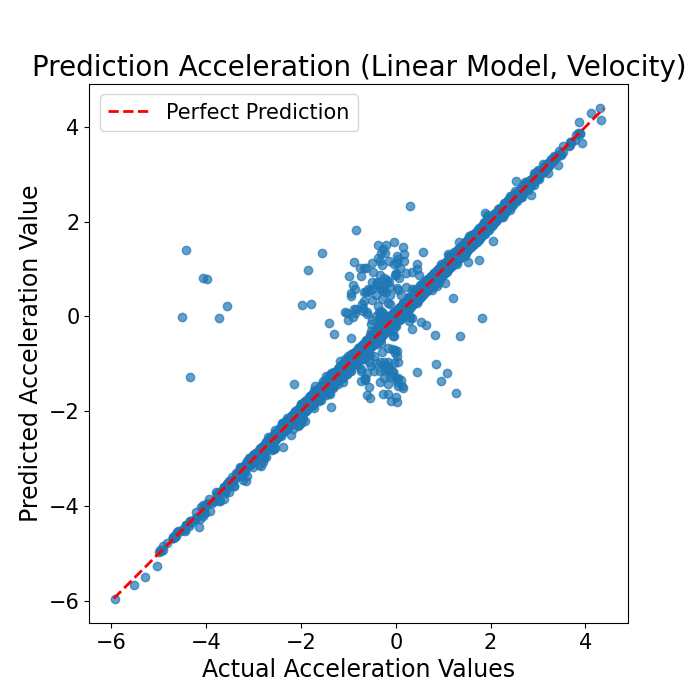
\includegraphics[width=\columnwidth]{images/figures/Prediction Acceleration (Linear Model, Velocity).png}
        \caption{Prediction results Velocity Model}
        \label{fig:prediciton_acceleration_velocity}
    \end{minipage}
\end{figure}

The graph seems to fit our low MSE and MAE values, as all predicted points are lying close to the red line which indicates
a perfect prediction.
Interestingly we can see that most inaccuracies lie in the middle where the acceleration is close to zero.
Our hypothesis is, that if our acceleration is close to zero the model has the least amount of information for inference, leading
to a more scattered prediction in this region.

\subsection{Equivalence of accelerations}

Note that both results of the models look quite similar. 
This is due to the fact, that we specifically trained both models to fit the same dataset. 
The similarity can be seen in the following figure.
The left shows how the predicted accelerations of both our linear models match up, while on the right we can see how the 
accelerations match up for the previously used ballistic integration method

\begin{figure}[h]
    \centering
    \begin{minipage}[b]{0.45\columnwidth}
        \centering
        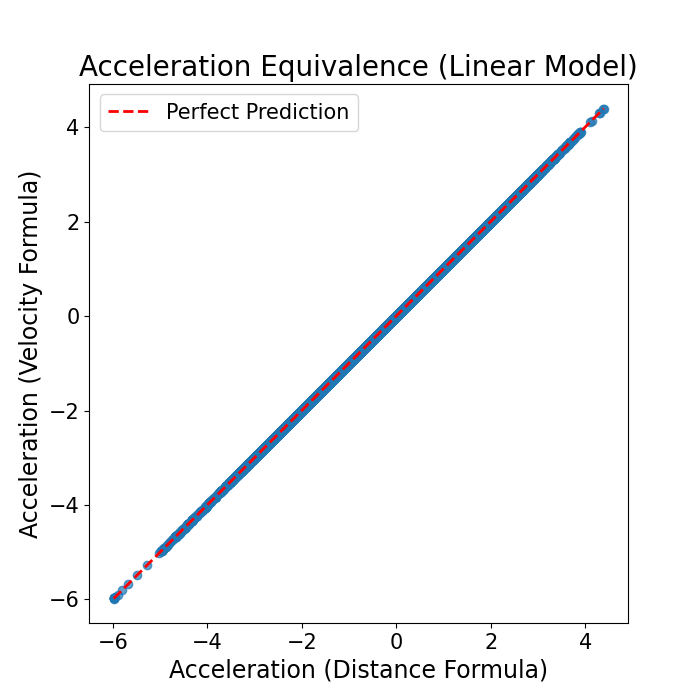
\includegraphics[width=\columnwidth]{images/figures/Acceleration Equivalence (Linear Model).png}
        \caption{Acceleration equivalence using linear model}
    \end{minipage}
    \hfill
    \begin{minipage}[b]{0.45\columnwidth}
        \centering
        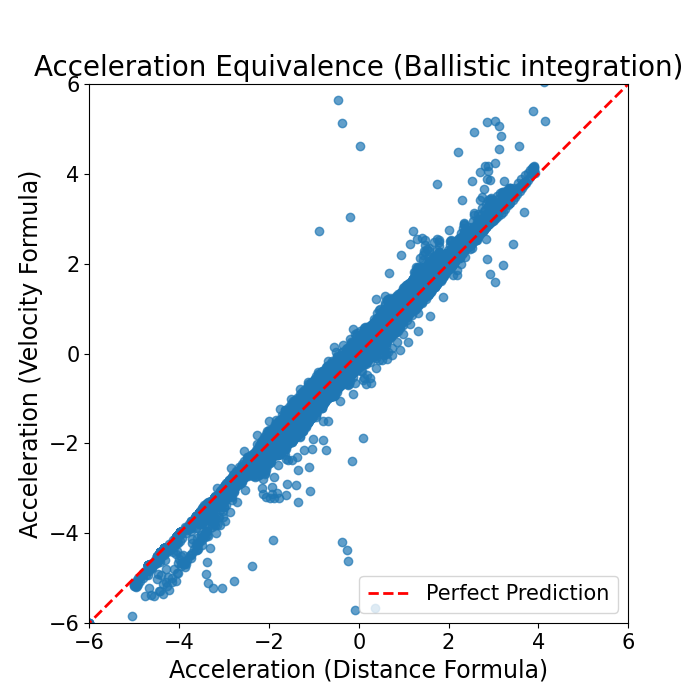
\includegraphics[width=\columnwidth]{images/figures/Acceleration Equivalence (Ballistic integration).png}
        \caption{Acceleration equivalence using ballistic model}
    \end{minipage}
    \caption{Caption for the entire figure}
\end{figure}

In the following, we can see the metrics of our results for the equivalence of the accelerations

\begin{table}[htbp]
\centering
\caption{Model Performance Comparison}
\label{tab:model_comparison_lin_v_bal}
\begin{tabular}{lccc}
\toprule
Model & MSE & MAE \\
\midrule
Linear Model & 1.8141e-06 & 7.5061e-04 \\
Ballistic Integration & 2.0698e+02 & 5.0158e-01 \\
\bottomrule
\end{tabular}
\end{table}

We can see that the accelerations from both our linear models match up almost perfectly, while the 
results from our previously used model are more scattered. 

\subsection{Prediction of the movement}
Using the coefficients determined by the linear regression we can rearrange the model such that the model predicts 
the distance (\ref{eq:distance_matrix}) and the velocity (\ref{eq:velocity_matrix}).
The following shows metrics for the prediction of the distance and the velocity using the coefficients.

\begin{table}[h]
    \centering
    \caption{Regression Metrics}
    \begin{tabular}{lccc}
    \toprule
 & {MSE} & {MAE} & {$R^2$ Score} \\
    \midrule
    Distance Formula & $1.3867 \times 10^{1}$ & $3.7239 \times 10^{0}$ & $9.8926 \times 10^{-1}$ \\
    Velocity Formula & $2.2635 \times 10^{0}$ & $1.5045 \times 10^{0}$ & $9.3378 \times 10^{-1}$ \\
    \bottomrule
    \end{tabular}
    \label{tab:regression_metrics}
\end{table}


As we can see, all metrics are quite low for both formulas. 
Though, our prediction for the distance and velocity is not perfect. 
For a better understanding, we also visualized our findings

\begin{figure}[htbp]
    \centering
    \begin{minipage}[b]{0.45\columnwidth}
        \centering
        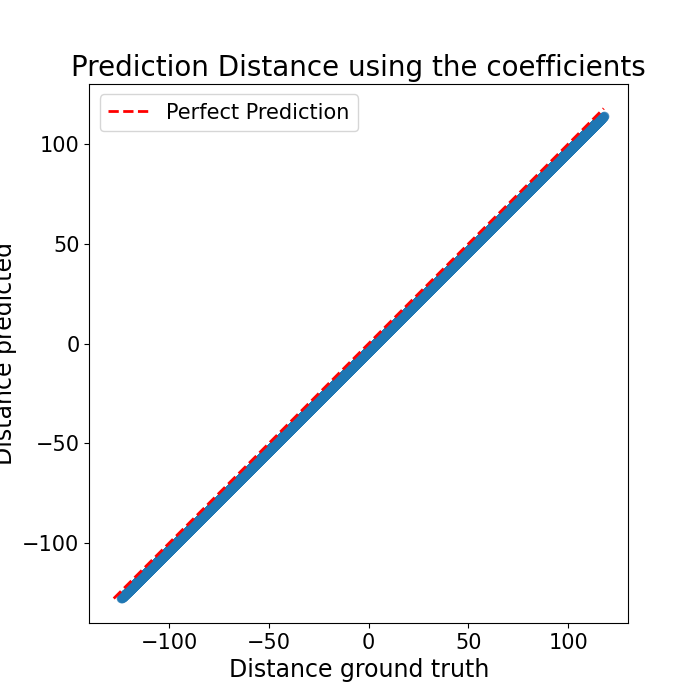
\includegraphics[width=\columnwidth]{images/figures/Prediction Distance using the coefficients.png}
        \caption{Prediction of the distance using coefficients}
        \label{fig:minipage3}
    \end{minipage}
    \hfill
    \begin{minipage}[b]{0.45\columnwidth}
        \centering
        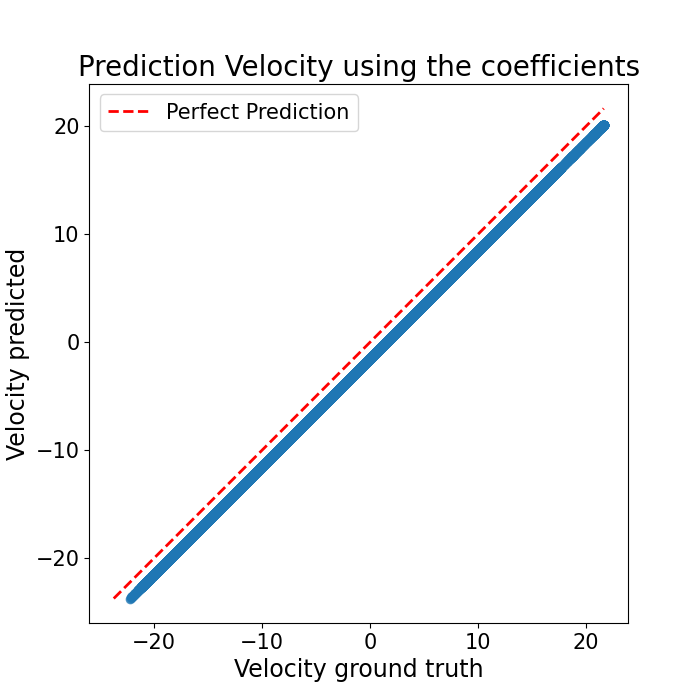
\includegraphics[width=\columnwidth]{images/figures/Prediction Velocity using the coefficients.png}
        \caption{Prediction of the velocity using coefficients}
        \label{fig:minipage4}
    \end{minipage}
    \label{fig:combined_figure_2}
\end{figure}

Again, we can see that the prediction matches up with the ground truth well.
Although we can see a small offset to the red line, especially on the velocity formula, our results might be sufficient for our use case.
These results can then be visualized using the drone-dataset-tool provided with the dataset.
Results comparing the prediction of the moving cars to the ground truth can be found \href{https://github.com/avocadoali/social_ai_practical_course}{here}.

